\documentclass[11pt]{article} \setlength{\oddsidemargin}{0in}
\setlength{\evensidemargin}{0in} \setlength{\textwidth}{6.5in}
\setlength{\parindent}{0in} \setlength{\textwidth}{16cm}
\setlength{\topmargin}{1in} \addtolength{\topmargin}{-1.5in}
\setlength{\textheight}{23cm} \setlength{\parskip}{0.75cm}

% Brackets
\usepackage{mathtools} \DeclarePairedDelimiter\ceil{\lceil}{\rceil}
\DeclarePairedDelimiter\floor{\lfloor}{\rfloor}

% Tikz settings
\usepackage{tikz} \usetikzlibrary{trees} \usetikzlibrary {positioning}
\definecolor {mypurple}{cmyk}{0.6,0.4,0.1,0} \definecolor
{myred}{cmyk}{0,0.3,0.3,0} \usetikzlibrary{fit,shapes.misc}

% Typesetting options
\usepackage{fancyvrb} \usepackage{amsmath,amsfonts,amssymb}
\usepackage [english]{babel} \usepackage [autostyle, english =
american]{csquotes} \usepackage[none]{hyphenat} \usepackage{url}

% Graph
\usepackage{tikz}


\usepackage{graphicx}
\graphicspath{ {images/} }

\begin{document}

\noindent CSCI 3104 Spring 2018 \hfill Problem Set 7\\
Cole Schlisner (03/10)

\hrulefill

{\fontfamily{cmr}\selectfont

  % ******************* PROBLEM 1 *********************
  \section*{Problem 1}

  \textit{(45 pts) Recall that the string alignment problem takes as
    input two strings $x$ and $y$, composed of symbols
    $x_i , y_j \in \Sigma$, for a fixed symbol set $\Sigma$, and returns a
    minimal-cost set of edit operations for transforming the string
    $x$ into string $y$.}

  \textit{Let $x$ contain $n_x$ symbols, let $y$ contain $n_y$
    symbols, and let the set of edit operations be those defined in
    the lecture notes (substitution, insertion, deletion, and
    transposition).}

  \textit{Let the cost of \textbf{indel} be 1, the cost of
    \textbf{swap} be 13 (plus the cost of the two sub ops), and the
    cost of \textbf{sub} be 12, except when $x_i = y_j$ , which is a
    “no-op” and has cost 0.}

  \textit{In this problem, we will implement and apply three
    functions.}

  \begin{enumerate}
  \item[(i)] \textit{ \texttt{alignStrings(x,y)} takes as input two
      ASCII strings $x$ and $y$, and runs a dynamic programming
      algorithm to return the cost matrix $S$, which contains the
      optimal costs for all the subproblems for aligning these two
      strings.  }

\begin{verbatim}
alignStrings(x,y) :  // x,y are ASCII strings
  S = table of length nx by ny // for memoizing the subproblem costs
  initialize S      // fill in the basecases
  for i = 1 to nx {
    for j = 1 to ny {
      S[i,j] = cost(i,j) // optimal cost for x[0..i] and y[0..j]
  }}
  return S
\end{verbatim}

  \item[(ii)] \textit{\texttt{extractAlignment(S,x,y)} takes as input
      an optimal cost matrix $S$, strings x, y, and returns a vector a
      that represents an optimal sequence of edit operations to
      convert x into y. This optimal sequence is recovered by finding
      a path on the implicit DAG of decisions made by
      \texttt{alignStrings} to obtain the value $S[n_x , n_y]$,
      starting from $S[0, 0]$.}

\begin{verbatim}
extractAlignment(S,x,y) : // S is an optimal cost matrix from alignStrings
  initialize a            // empty vector of edit operations
  [i,j] = [nx,ny]         // initialize the search for a path to S[0,0]
  while i > 0 or j > 0
    a[i] = determineOptimalOp(S,i,j,x,y) // what was an optimal choice?
    [i,j] = updateIndices(S,i,j,a) // move to next position
  }
  return a
\end{verbatim}

    \textit{When storing the sequence of edit operations in
      \texttt{a}, use a special symbol to denote no-ops.}

  \item[(iii)] \textit{\texttt{commonSubstrings(x,L,a)} which takes as
      input the ASCII string x, an integer $1 \le L \le n_x$, and an
      optimal sequence a of edits to x, which would transform x into
      y. This function returns each of the substrings of length at
      least L in x that aligns exactly, via a run of no-ops, to a
      substring in y.}
  \end{enumerate}

  \begin{enumerate}
  \item[(a)] \textit{From scratch, implement the functions
      \texttt{alignStrings}, \texttt{extractAlignment}, and
      \texttt{commonSubstrings}. You may not use any library functions
      that make their implementation trivial. Within your
      implementation of \texttt{extractAlignment}, ties must be broken
      uniformly at random.}

    \textit{Submit (i) a paragraph for each function that explains how
      you implemented it (describe how it works and how it uses its
      data structures), and (ii) your code implementation, with code
      comments.}

    \textit{Hint: test your code by reproducing the \texttt{APE} /
      \texttt{STEP} and the \texttt{EXPONENTIAL} / \texttt{POLYNOMIAL}
      examples in the lecture notes (to do this exactly, you’ll need
      to use unit costs instead of the ones given above).}
    \pagebreak
    \\\\
    \textbf{alignStrings:}
    This implementation is essentially the same algorithm as the pseudocode provided, except instead of using a separate function cost(i,j) to determine the optimal subproblem cost it just stores the subproblem costs in an array and picks the minimum. 
    The specific subproblems stored in the cost array (added with their respective costs) are S[i-2][j-2] (Swap), S[i-1][j-1] (Sub), S[i-1][j] (Delete), S[i][j-1] (Insert). S[i][j], the current subproblem is set to the minimum of these. 
    The algorithm first initializes S with the base cases (first column and first row), and then computes each row sequentially using the previous entries in the table. \\\\
    \textit{python 3.6:}
    \begin{verbatim}
    def alignStrings(x,y):
      costS = 12
      costT = 13
      costID = 1

      # Y on top, X on side as in example
      S = [[0 for j in range(len(y)+1)] for i in range(len(x)+1)]
      
      # base cases = cost of aligning empty strings 
      for j in range(len(y)+1):
        S[0][j] = j
      for i in range(len(x)+1):
        S[i][0] = i

      for i in range(1,len(x)+1):
        for j in range(1,len(y)+1):
          cost = []
          
          # Swap -- i-2,j-2
          if j > 1 and i > 1:
            cost.append(S[i-2][j-2] + costT
                  + (0 if (x[i-1] == y[j-2]) else 1)
                  + (0 if (y[j-1] == x[i-2]) else 1))
          
          # Sub -- i-1,j-1
          cost.append(S[i-1][j-1] + (costS if x[i-1] != y[j-1] else 0))
          
          # insert -- i,j-1
          cost.append(S[i][j-1] + costID)
          
          # delete -- i-1,j
          cost.append(S[i-1][j] + costID)
          
          S[i][j] = min(cost)
      return S
    \end{verbatim}
    \pagebreak

    \textbf{extractAlignment:}
    This implementation works in largely the same way that alignStrings works -- by looking at each relevant subproblem and picking the minimum. The differences are that (a) this is done in reverse and (b) instead of setting S[i][j] to this minimum value, we record which subproblem the minimum came from (using the \textit{ops} array) and then set the coordinates i and j to the coordinates of the subproblem. Specifically, this algorithm records the indicies of all subproblems with the minimum value within the cost array and picks one at random. This allows the algorithm to break ties evenly if there are two or more subproblems that yield the same optimal solution. My implementation also records the indicies of the chosen subproblems in an array (\textit{optimalpath}) so that the path of the extracted alignment can be visualized easily. \\
    \textit{python 3.6 (next page):}
    \pagebreak
    \begin{verbatim}
    import random
    def extractAlignment(S,x,y):
      costS = 12
      costT = 13
      costID = 1
      optimaledits = []
      optimalpath = [[0 for j in range(len(y)+1)] for i in range(len(x)+1)]
      i = len(x)
      j = len(y)
      while i > 0 or j > 0:
        optimalpath[i][j] = 1
        # build cost array of tuples = (symbol, cost)   
        cost = []
        cost.append(("s", S[i-1][j-1] + (costS if x[i-1] != y[j-1] else 0))) 
        cost.append(("i", S[i][j-1] + costID))
        cost.append(("d", S[i-1][j] + costID))
        if j > 1 and i > 1:
          cost.append(("t", S[i-2][j-2] + costT 
                  + (0 if (x[i-1] == y[j-2]) else 1)
                  + (0 if (y[j-1] == x[i-2]) else 1)))
        # the current optimal value is the minimum of cost
        optval = S[i][j]
        
        # choose one of the edits at random that have the same cost 
        # as the current optimal value 
        opt = random.choice([c[0] for c in cost if c[1] == optval])
        
        # if the characters in both strings were the same (and it was a sub),
        # then insert "|" (no-op) at the beginning of the list
        if (opt == "s" and x[i-1] == y[j-1]):
          optimaledits.insert(0, "|")

        # otherwise insert the operation 
        else: optimaledits.insert(0,opt)
        
        # update the indicies to the selected subproblem
        if opt == "s":
          i -= 1
          j -= 1
        elif opt == "i":
          j -= 1
        elif opt == "d":
          i -= 1
        elif opt == "t":
          optimaledits.insert(0,opt)
          i -= 2
          j -= 2
      return optimaledits, optimalpath
  \end{verbatim}

  \textbf{commonSubstrings:}
  This implementation of commonSubstrings() simply scans through the list of edit operations \textit{a}, and looks for the no-op character "$\vert$". Once this is found it adds the corresponding character in X (which is the same in Y) to the last substring in an array of common substrings. For each sequential "$\vert$" in \textit{a}, the same thing is done, until an edit operation in \textit{a} is found which is not a no-op ("$\vert$"), then the algorithm adds a new empty string to the list of common substrings. Now, if another no-op sequence is found, the characters will be added to this new empty string. The algorithm will add all common substrings to the array, and then return a filtering of this array by length L. \\
  \textit{python 3.6:}
  \begin{verbatim}
  def commonSubstrings(x,L,a):
    substr = [""]
    for i in range(len(a)):
      if a[i] == "|":
        substr[-1] += x[i]
      else: 
        substr.append("")
    return [s for s in substr if len(s) >= L]
  \end{verbatim}

  \pagebreak

  \item[(b)] \textit{Using asymptotic analysis, determine the running
      time of the call $$\texttt{commonSubstrings(x, L,
        extractAlignment( alignStrings(x,y), x,y ) )}$$ Justify your
      answer.}
    \\\\
    \begin{itemize}
    \item The first function called within this call is \textit{alignStrings} -- the running time of alignStrings is $O(n_xn_y)$, as each entry in the ($n_x$ x $n_y$) table is calculated in constant time (the process of picking the minimum of the previous optimal solutions). The cost of the setup before these calculations is $\Theta(n_xn_y) + \Theta(n_x) + \Theta(n_y)$ and thus does not contribute to the total running time. 
    \item The second function call is \textit{extractAlignment} -- this takes $O(n_y+n_x)$ time in the worst case, which corresponds to deleting the input string X and inserting the target string Y. In terms of the cost table, this would require the algorithm to visit (and do a constant time operation on) each entry along the perimeter of the table (i.e. the longest path from S[i,j] to S[0,0]). In the best case, the input string and the target string are the same and \textit{extractAlignment} takes $O(n_y)$ -- the cost of visiting each entry along the diagonal (a series of no-ops). 
    \item The final function call is \textit{commonSubstrings} -- this will take $\Theta(n_a)$, as it is a simple loop through the edit operations array (plus another loop through the created substrings array to filter by length).
    \end{itemize}

    Thus the total running time of the call would be $O(n_xn_y) + O(n_x + n_y))$ = $O(n_xn_y)$
    
    \pagebreak

  \item[(d)] \textit{String alignment algorithms can be used to detect
      changes between different versions of the same document (as in
      version control systems) or to detect verbatim copying between
      different documents (as in plagiarism detection systems).  The
      two \texttt{data\_string} files for PS7 (see class Moodle)
      contain actual documents recently released by two independent
      organizations. Use your functions from (1a) to align the text of
      these two documents. Present the results of your analysis,
      including a reporting of all the substrings in x of length
      $L = 9$ or more that could have been taken from y, and briefly
      comment on whether these documents could be reasonably
      considered original works, under CU's academic honesty policy.}
    \\    
    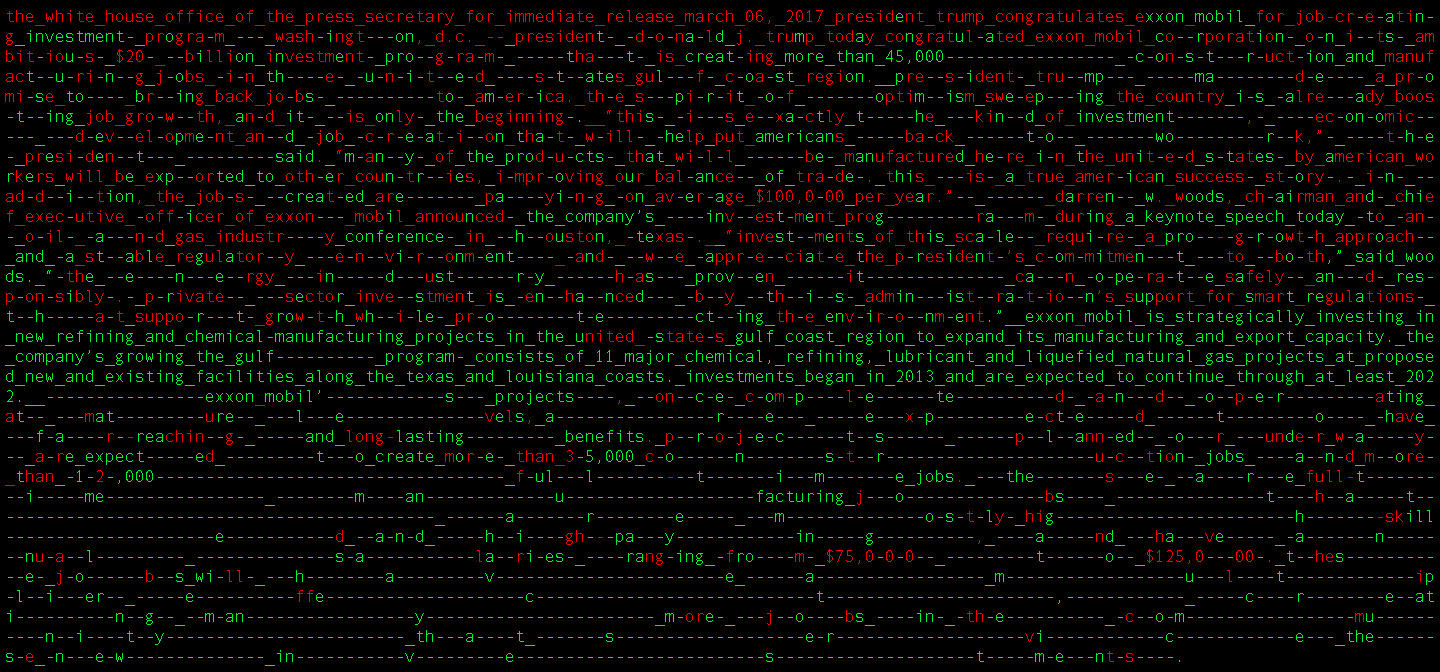
\includegraphics[width=15cm,height=5cm]{1d}

    This is the input string (x.txt) formatted so that green characters are those which were kept via no-ops, and the red characters are characters that were deleted. Dashes represent insertions, and underscores represent spaces. It is immediately apparent that a large portion of the text was identical, however here are the common substrings of length at least 9:

    \begin{itemize}
      \item "manufacturing "
      \item " gulf coast "
      \item "the company's "
      \item " a keynote speech today "
      \item "conference"
      \item "," said woods. ""
      \item "."  exxon"
      \item "mobil is strategically investing in new refining and chemical-manufacturing projects in the u"
      \item " gulf coast region to expand its manufacturing and export capacity. the company’s growing the gulf"
      \item " consists of 11 major chemical, refining, lubricant and liquefied natural gas projects at proposed new and existing facilities along the texas and louisiana coasts. investments began in 2013 and are expected to continue through at least 2022. "
      \item " to create "
      \item "facturing "
    \end{itemize}

    This would classify as a violation of the honor policy, as the news article quoted the press release without citing the source. 

  \end{enumerate}

  \newpage

  % ******************* PROBLEM 2 *********************
  \section*{Problem 2}

  \textit{(20 pts) Ron and Hermione are having a competition to see
    who can compute the $n$th Pell number $P_n$ more quickly, without
    resorting to magic. Recall that the $n$th Pell number is defined
    as $P_n = 2 P_{n-1} + P_{n-2}$ for $n > 1$ with base cases
    $P_0 = 0$ and $P_1 = 1$.  Ron opens with the classic recursive
    algorithm:}

\begin{verbatim}
Pell(n):
  if n == 0 { return 0 }
  else if n == 1 { return 1 }
  else { return 2*Pell(n-1) + Pell(n-2) }
\end{verbatim}

  \begin{enumerate}
  \item[(a)]{\textit{Hermione counters with a dynamic programming
        approach that “memoizes” (a.k.a.  memorizes) the intermediate
        Pell numbers by storing them in an array $P[n]$. She claims
        this allows an algorithm to compute larger Pell numbers more
        quickly, and writes down the following
        algorithm. \footnote{Ron briefly whines about Hermione's
          \texttt{L[n]=undefined} trick (``an unallocated array!''),
          but she point out that \texttt{MemLuc(n)} can simply be
          wrapped within a second function that first allocates an
          array of size $n$, initializes each entry to undefined, and
          then calls \texttt{MemLuc(n)} as given.}}}

\begin{verbatim}
MemPell(n) {
  if n == 0 { return 0 } else if n == 1 { return 1 }
  else {
    if (P[n] == undefined) { P[n] = 2*MemPell(n-1) + MemPell(n-2) }
    return P[n]
  }
}
\end{verbatim}

    \begin{enumerate}
    \item[i.] \textit{Describe the behavior of \texttt{MemPell(n)} in
        terms of a traversal of a computation tree. Describe how the
        array \texttt{P} is filled.}
    \item[ii.] \textit{Determine the asymptotic running time of
        \texttt{MemPell}. Prove your claim is correct by induction on
        the contents of the array.}
    \end{enumerate}
    \begin{enumerate}
      \item[i.] If MemPell(n-1) is the left subtree, and MemPell(n-2) is the right, then the computation would look like a post-order traversal because it computes all of the (n-1) terms down to the base case, and then computes each corresponding (n-2) term before returning. The array is filled sequentially from the beginning to the end starting from the base cases. 
      \item[ii.] Because of the post-order traversal, each P[n] for n $\in$ [2..n] is calculated before anything else in the tree, which memoizes all pell numbers $\le$ n. Thus there is no computation left to do for the rest of the tree. Thus the running time must be O(n).
    \end{enumerate}
    \pagebreak
  \item[(b)] \textit{Ron then claims that he can beat Hermione's
      dynamic programming algorithm in both time and space with
      another dynamic programming algorithm, which eliminates the
      recursion completely and instead builds up directly to the final
      solution by filling the P array in order. Ron's new algorithm
      \footnote{Ron is now using Hermione's undefined array trick;
        assume he also uses her solution of wrapping this function
        within another that correctly allocates the array.} is}

\begin{verbatim}
DynPell(n) :
  P[0] = 0, P[1] = 1
  for i = 2 to n { P[i] = 2*P[i-1] + P[i-2] }
  return P[n]
\end{verbatim}

    Determine the time and space usage of \texttt{DynPell(n)}. Justify
    your answers and compare them to the answers in part (2a).
    \\\\
    \textbf{T(n)} = O(n), because the loop is executed n-2 times, each time doing a constant-time operation.\\
    \textbf{S(n)} = O(n), as the array is exactly n elements.\\
    This is exactly the same time and space cost as Hermoine's algorithm. The array is even filled in in the same order. 
    \\
  \item[(c)] \textit{With a gleam in her eye, Hermione tells Ron that
      she can do everything he can do better: she can compute the
      $n$th Pell number even faster because intermediate results do
      not need to be stored. Over Ron's pathetic cries, Hermione says}

\begin{verbatim}
FasterPell(n) :
  a = 0, b = 1
  for i = 2 to n
    c = 2 * a + b
    a = b
    b = c
  end
  return a
\end{verbatim}

    Ron giggles and says that Hermione has a bug in her
    algorithm. Determine the error, give its correction, and then
    determine the time and space usage of
    \texttt{FasterPell(n)}. Justify your claims.
    \\\\
    \textbf{error:} c = 2 * a + b \\
    \textbf{correction:} c = 2 * b + a \\
    \textbf{T(n)}= O(n) - this is a simple loop doing three O(1) operations n-2 times \\
    \textbf{S(n)}= O(1) - only three numbers are stored at any given time.  
  \pagebreak
  \item[(d)] \textit{In a table, list each of the four algorithms as
      columns and for each give its asymptotic time and space
      requirements, along with the implied or explicit data structures
      that each requires. Briefly discuss how these different
      approaches compare, and where the improvements come from. (Hint:
      what data structure do all recursive algorithms implicitly
      use?)}
    \\\\
    \begin{tabular}{ |p{3cm}||p{2cm}|p{2cm}|p{2cm}|p{2cm} }
     \hline
      & Pell(n) & MemPell(n) & DynPell(n) & FasterPell(n)\\
     \hline
     \hline
     Running Time   & O($2^n$)    & O(n)&  O(n) & O(n)\\
     \hline
     Space &   O(1)  & O(n) & O(n)  & O(1)\\
     \hline
     Data Structs& Tree & Array/Tree& Array & None \\
     \hline
    \end{tabular}
    \\\\
    MemPell improves upon Pell by memoizing results in the computation tree - all of the pell numbers are computed along the left subtree. This is an improvement in time at the cost of space. DynPell does not improve upon MemPell in time or space. FasterPell is an improvement on DynPell/MemPell because it uses the same method of calculation without memoizing the intermediate results - this is like only using the last 3 rows in the napsack problem. 

  \item[(e)] \textit{(5 pts extra credit) Implement
      \texttt{FasterPell} and then compute $P_n$ where n is the
      four-digit number representing your MMDD birthday, and report
      the first five digits of $P_n$. Now, assuming that it takes one
      nanosecond per operation, estimate the number of years required
      to compute $P_n$ using Ron's classic recursive algorithm and
      compare that to the clock time required to compute $P_n$ using
      FasterPell.}
    \\\\
    First 5 digits of $P_{0828}=P_{828}$: 14916 \\\\
    Number of years for good ol' ronny boy's algorithm: $2^{828}$ns = 5.672*$10^{232}$ years (according to Wolfram alpha) \\\\
    Real time according to unix: 0m0.240s
  \end{enumerate}
  % ---------------------------------------------------
  \newpage

\textbf{References} \\
\hrulefill
\begin{enumerate}
  \item CLRS
\end{enumerate}
\end{document}